% !TeX root = main.tex


\documentclass[a4paper,12pt]{article}
\usepackage[french]{babel} %translates document elements to french
\usepackage{Arnaud_C_rds}

\hypersetup{pdftitle={L3 Internship report},
pdfauthor={Arnaud COSTERMANS},
pdfcreationdate=D:20240430133559+01’00’,
pdfsubject={Internship report},
pdfkeywords={Internship, L3, SOMAIR, CanOP, Uranium extraction, Orano Mining},
}






\setlength{\parskip}{0.5 em} %adjust the space between paragraphes to be a bit wider


%example figure
% \begin{figure}
%     \centering
%     \includegraphics[width=0.5\textwidth]{example.png}
%     \caption{Here goes your caption}
%     \label{here goes the label to be able to refrence it}
% \end{figure}



% Page de garde
\begin{document}
%on repartie le document en plusieure fichier Tex pour faciliter le lecture
\begin{titlepage}
    \centering
    
    % Logo de l'Institut
    
\includegraphics[width=0.3\textwidth]{img/logo/logo_institut.jpeg} 
\includegraphics[width=0.3\textwidth]{img/logo/UPSaclay.jpg}

    % Titre du sujet
    \vspace{1.5cm}
    {\LARGE\textbf{Rapport de stage}\par}
    
    % Informations sur l'étudiant
    \vspace{1.5cm}
    {\large\textbf{Arnaud COSTERMANS}\par}
    
    % Année universitaire
    \vspace{0.5cm}
    Année universitaire : 2023-2024
    
    % Année d'études et nom de l'Institut
    \vspace{0.5cm}
    Année d'études : Promotion 2024 (L3) \\
    Licence de Science et Technologie \\
    Institut Villebon - \textit{Georges Charpak}
    
    % Informations sur le laboratoire/entreprise
    \vspace{2cm}
    
\includegraphics[width=0.2\textwidth]{img/logo/logo-orano.png}
    
    % Nom et adresse du laboratoire/entreprise
    \vspace{0.5cm}
    \textbf{Orano Mining}\\
    125 Av. de Paris, 92320 Châtillon\\
    % Nom du maître de stage
    \vspace{0.5cm}
    Maître de stage : Youcef BENSEDIK
    
    % Nom de l'enseignant référent
    \vspace{0.5cm}
    Enseignant référent : Cyril DAUPHIN
    
    % Durée du stage ou date de soutenance
    \vspace{0.5cm}
    Stage effectué du 22/04 au 13/06 (7 semaines)
\end{titlepage}
\clearpage

%\maketitle

\begin{center}

    \subsubsection*{Remerciement}
\addcontentsline{toc}{section}{Remerciement}
J'aimerais remercier Youcef BENSEDIK, qui bien que souvant occuper a toujour trouver le temps pour faire un point et m'expliquer quelque chose. J'aimerai egalement remercier Arnaud WUILBEAUX ainsi qu’Orano  de m'avoir accueilli pendant ce stage et tout les equipe qui m'on expliquer le fonctionement de certain chose, a la fois de la procedure a des methode de production.
\end{center}


\begin{abstract}
    \lipsum[1]
\end{abstract}
    

\begin{adjustwidth}{30pt}{30pt}
\end{adjustwidth}

% \vspace{50pt}
%remerciement 
\tableofcontents
% \newpage
\listoffigures
%\listoftables
\clearpage
\section{Introduction}
\lipsum[]



\section{Somaïr}
Dans cette partie, nous allons tout particulièrement nous intéresser au fonctionnement de Somaïr, la mine à ciel ouvert d'Orano au Niger, car c'est la qu'est déployé le projet CanOp et qui me faut comprendre leur procédure pour donner des suggestions cohérentes.
\subsection{L'exploration}
Avant le début de l'extraction, des géologues ont réalisé des études pour trouver d'éventuel gisement. S'ils soupçonnent la présence d'uranium, les géologues vont réaliser des campagnes de sondage successives\footnote{Soit une carotte ou un forage dans lequel on abaisser un 
sonde gamma. Cela permet d'etablire le gisment en 3D}. La maille de sondage sera à affiner jusqu'à avoir des forages espacés de 25~m. 
\subsection{L'extraction}
\label{ssec_extraction}
Si la décision de passer en production est prise alors on va venir enlever toute la roche au-dessus du gisement (50 a 70~m à Somaïr) et l’on va affiner le sondage jusqu'à une maille de 5~m*5~m qui va permettre de modéliser au mieux la distribution d'uranium dans le sol. Enfin, la fosse sera divisée en carrés de 2,5~m de large sur 2,5~m de longueur sur 0,5~m de profondeur que l'on appellera "slab" par la suite. Pour extraire ces slabs, on enterre juste assez d'explosif pour fragiliser la roche et permettre qu'une pelle mécanique puisse extraire la slab pour la charge dans un camion.
\subsection{Classification des slabs}
\begin{figure}
    
    \begin{subfigure}[t]{0.4\textwidth}
        \centering
        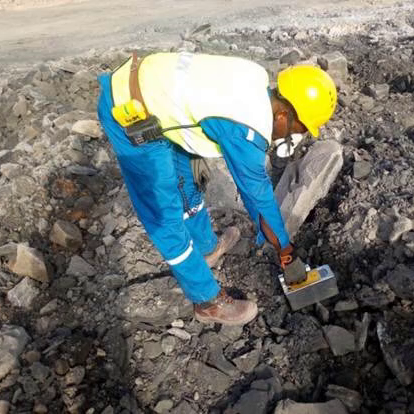
\includegraphics[height=0.3\paperwidth]{img/photo/Travail_geiger.png}
        \caption{Photo d'un operateur utilisant un compteur Geiger Müller pour mesurer la teneur en uranium d'un slab}
        \label{fig_AP_geiger}
    \end{subfigure}
    \begin{subfigure}[t]{0.6\textwidth}
        \centering
        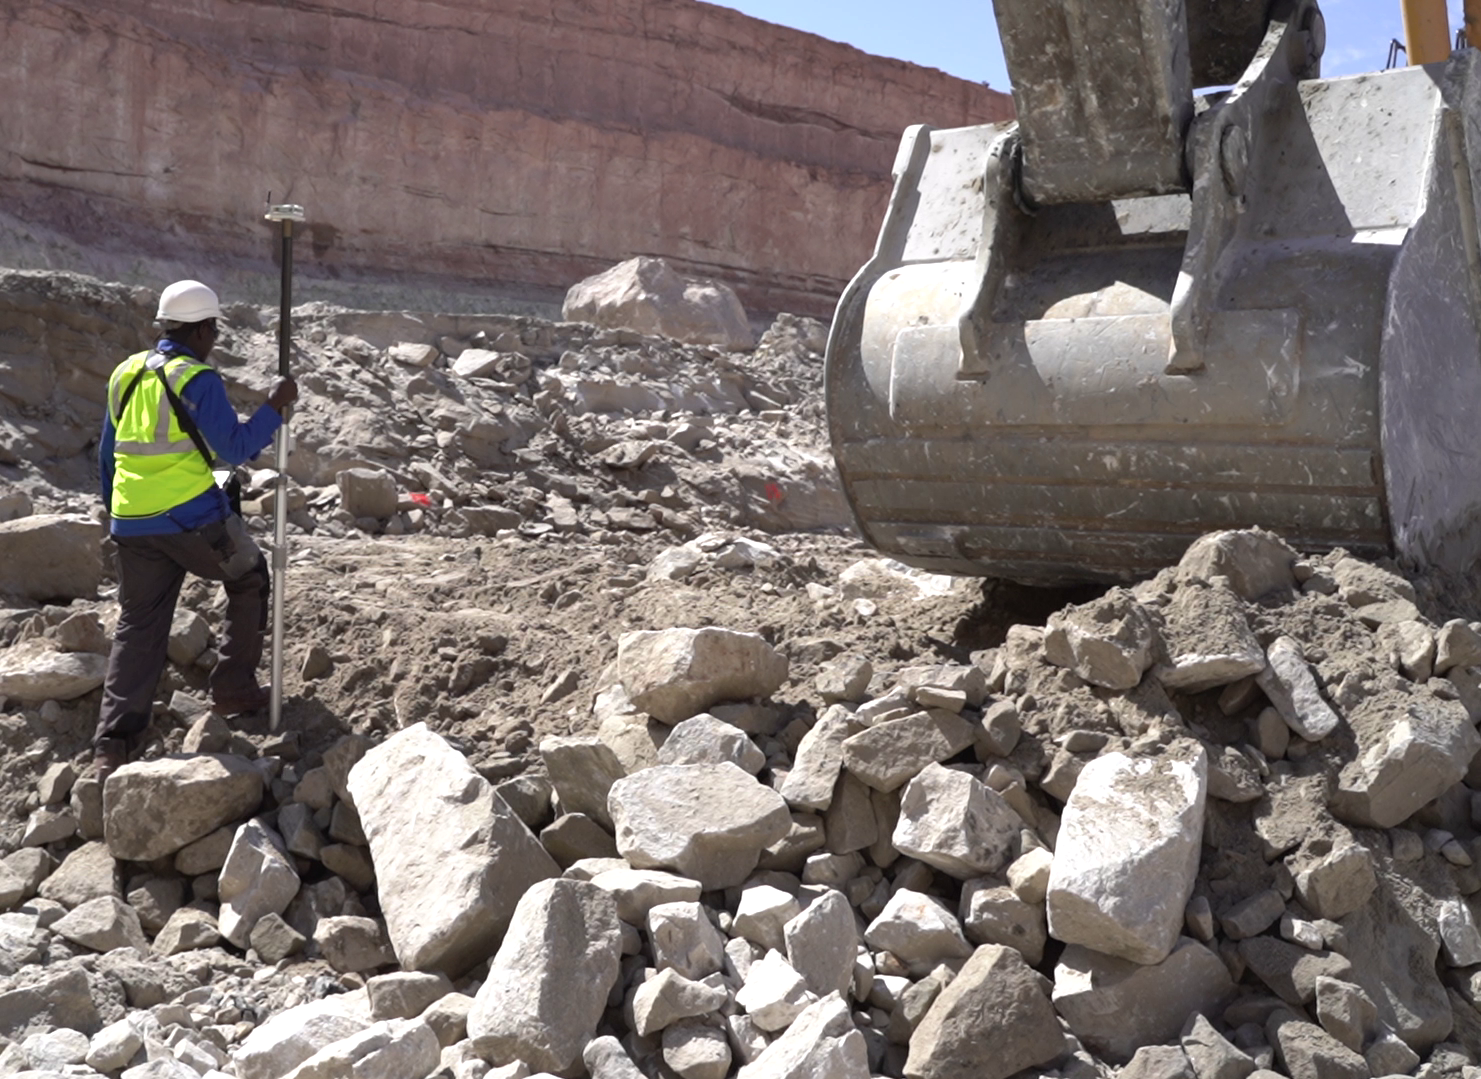
\includegraphics[height=0.3\paperwidth]{img/photo/CanOp_utilisation.png}
        \caption{Photo d'un operateur utilisant la CanOp pour mesurer la teneur en uranium d'un slab. Il porte une tablette pour voir les mesure et sa position en temps reel}
        \label{fig_AP_CanOp}
    \end{subfigure}
    \caption{Photo d'AP utilisant un compteur Geiger Müller et la CanOp}
\end{figure}
Pour savoir comment traiter ces slabs  après extraction, nous les catégorisons en 7~classes de M0 à  en fonction de leur teneur en uranium. Au début, ces teneurs étaient mesurées  Les slabs~M0 sont dites stériles, car elle contient tellement peu d'uranium que l'on ne souhaite pas les traiter. Les classes~M1 et M2 subissent un traitement que l'on dit statique, car c'est slab sont empiler et l’on attend que l'uranium descend par gravité jusqu'un bas. Enfin les slabs de classe supérieure reçoivent un traitement dynamique où en fonction de leur classe elles seront dissoutes avec plus ou moins d'acide selon leurs classes. Il est donc important de bien classer les slabs, car sinon, soit on gaspille  de l'acide ou alors il reste des l'uranium non extrait dans notre refus.
%TODO:mistakes
Avant, pour classer une slab, un Aide Prospecteur (AP) utiliser un compteur Geiger Müller en se penchant pour obtenir des mesures a plusieurs points sur le slab. Il était donc pénible de se pencher en permanence et donc en 2018 a été lancer le projet CanOp pour réduire la pénibilité de la tache.

\section{CanOp}
\label{sec_CanOp}
CanOp est le nom qui a été donné au projet de crée une sonde nouvelle génération pour la mine Somaïr au Niger. Cette sonde est composée de 3~pièces. 
\begin{itemize}
    \item 2 Sondes de rayonnement Gamma fournissent par la société Geovista
    \item une partie électronique qui inclue une batterie.
    \item Un GPS différentiel fourni par Ophelia 
\end{itemize}
Un opérateur utilise cette sonde en connexion avec une tablette pour déterminer ou extraire du minerai. 
\subsection{Les sondes Gamma}
\label{ssec_sonde}
Les sondes gamma de cet appareil proviennent de chez Ophelia et sont composées de deux parties.
\begin{figure}
    
    \begin{subfigure}{0.9\textwidth}
        \centering
        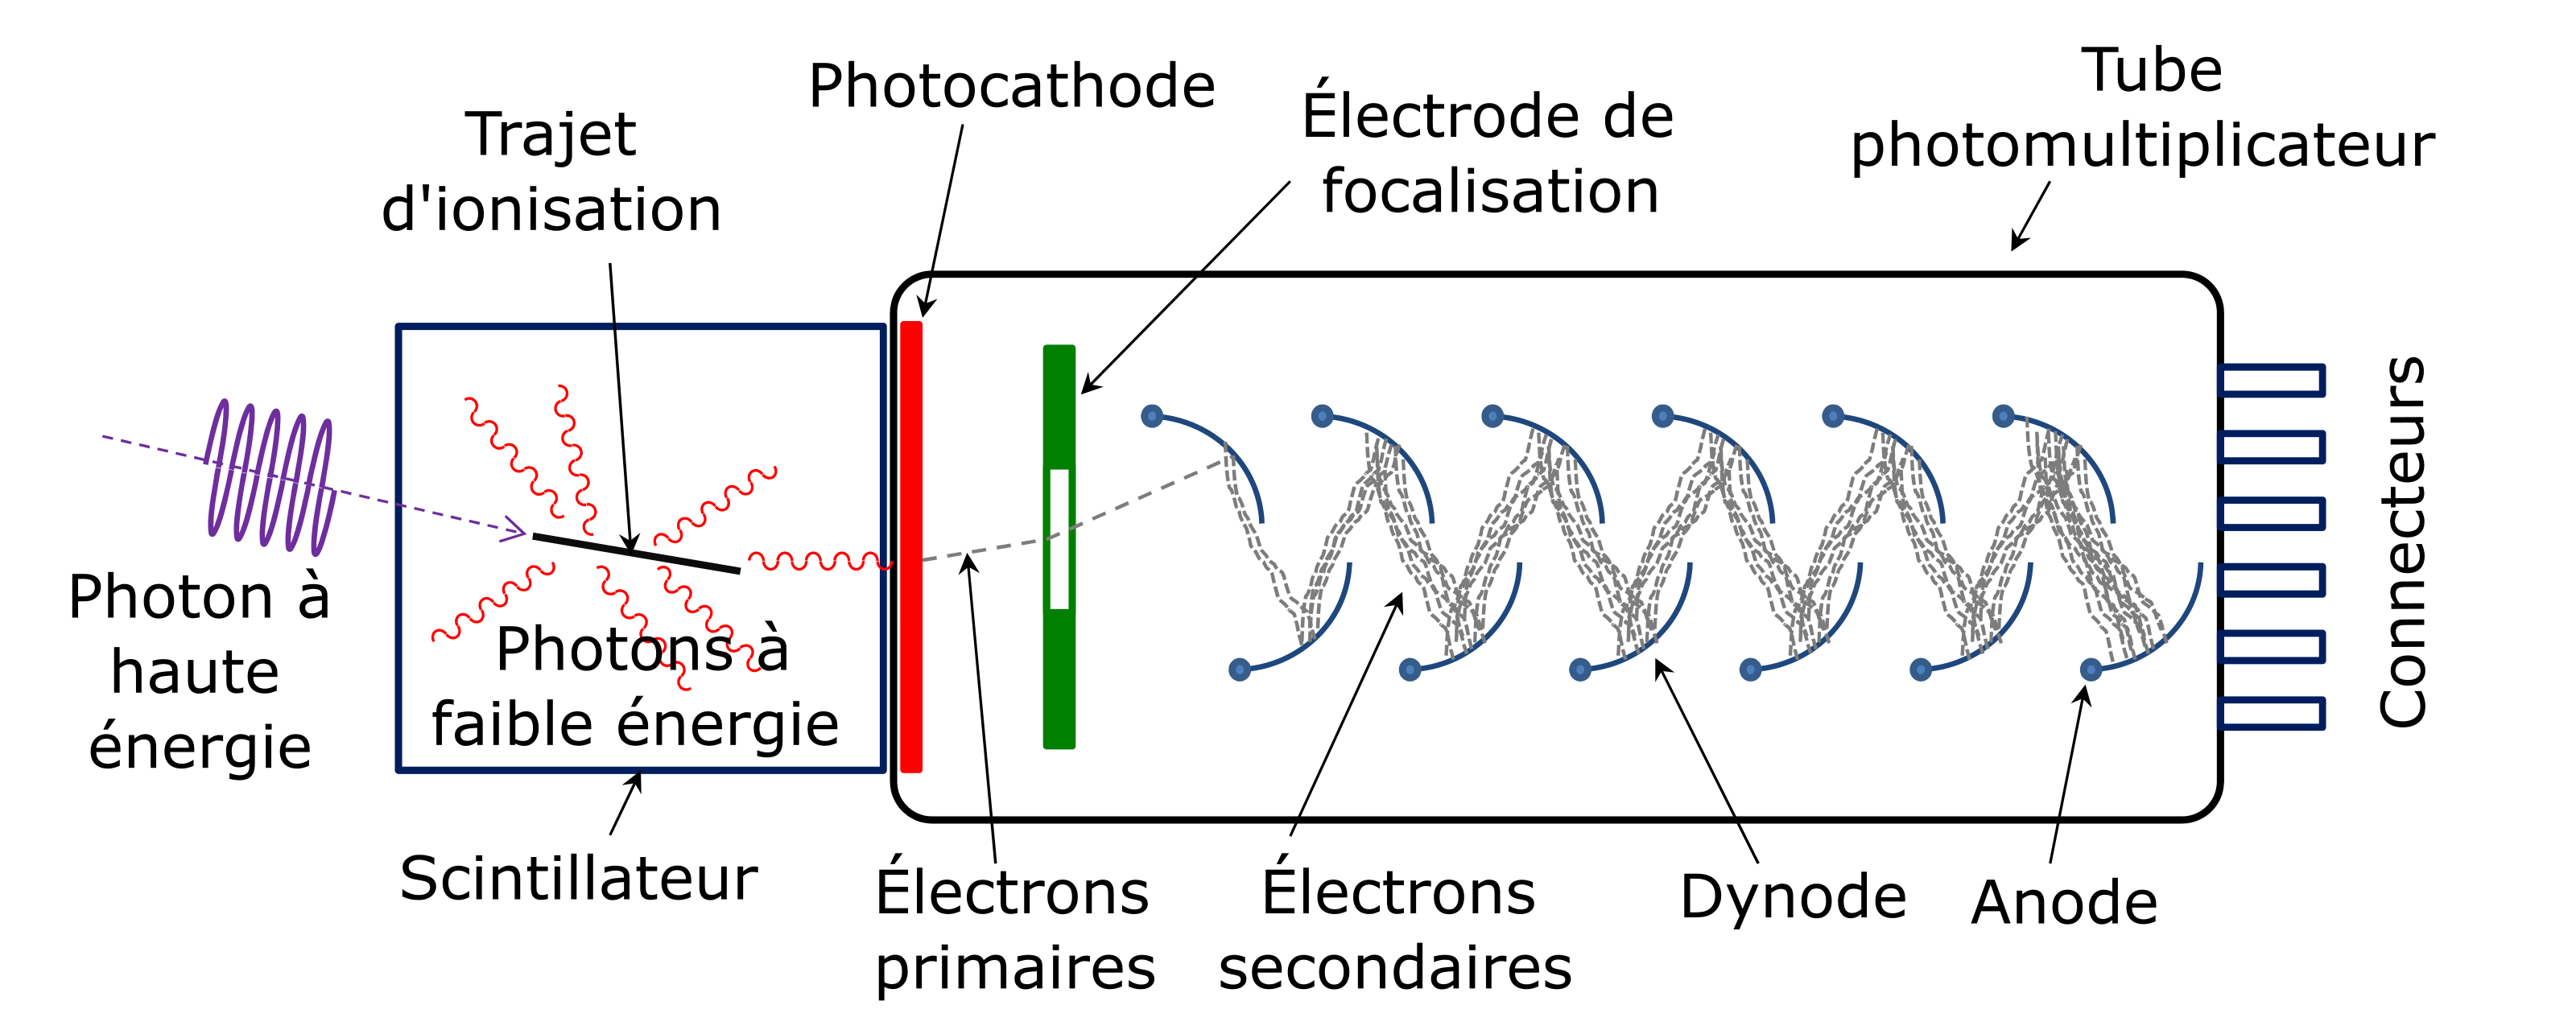
\includegraphics[width=0.9\textwidth]{img/she/Photomultiplier_coupled_to_a_scintillator_-_fr.png}
        \caption[Shema d'une sonde gamma NaI]{Schéma d'une sonde gamma NaI. Source~: \href{https://commons.wikimedia.org/wiki/File:Photomultiplier_coupled_to_a_scintillator_-_fr.png}{Qwerty123uiop}, \href{https://creativecommons.org/licenses/by-sa/3.0}{CC BY-SA~3.0}, via Wikimedia Commons}
        \label{fig_detecteur_gamma}
    \end{subfigure}
    \begin{subfigure}{0.45\textwidth}
        \centering
        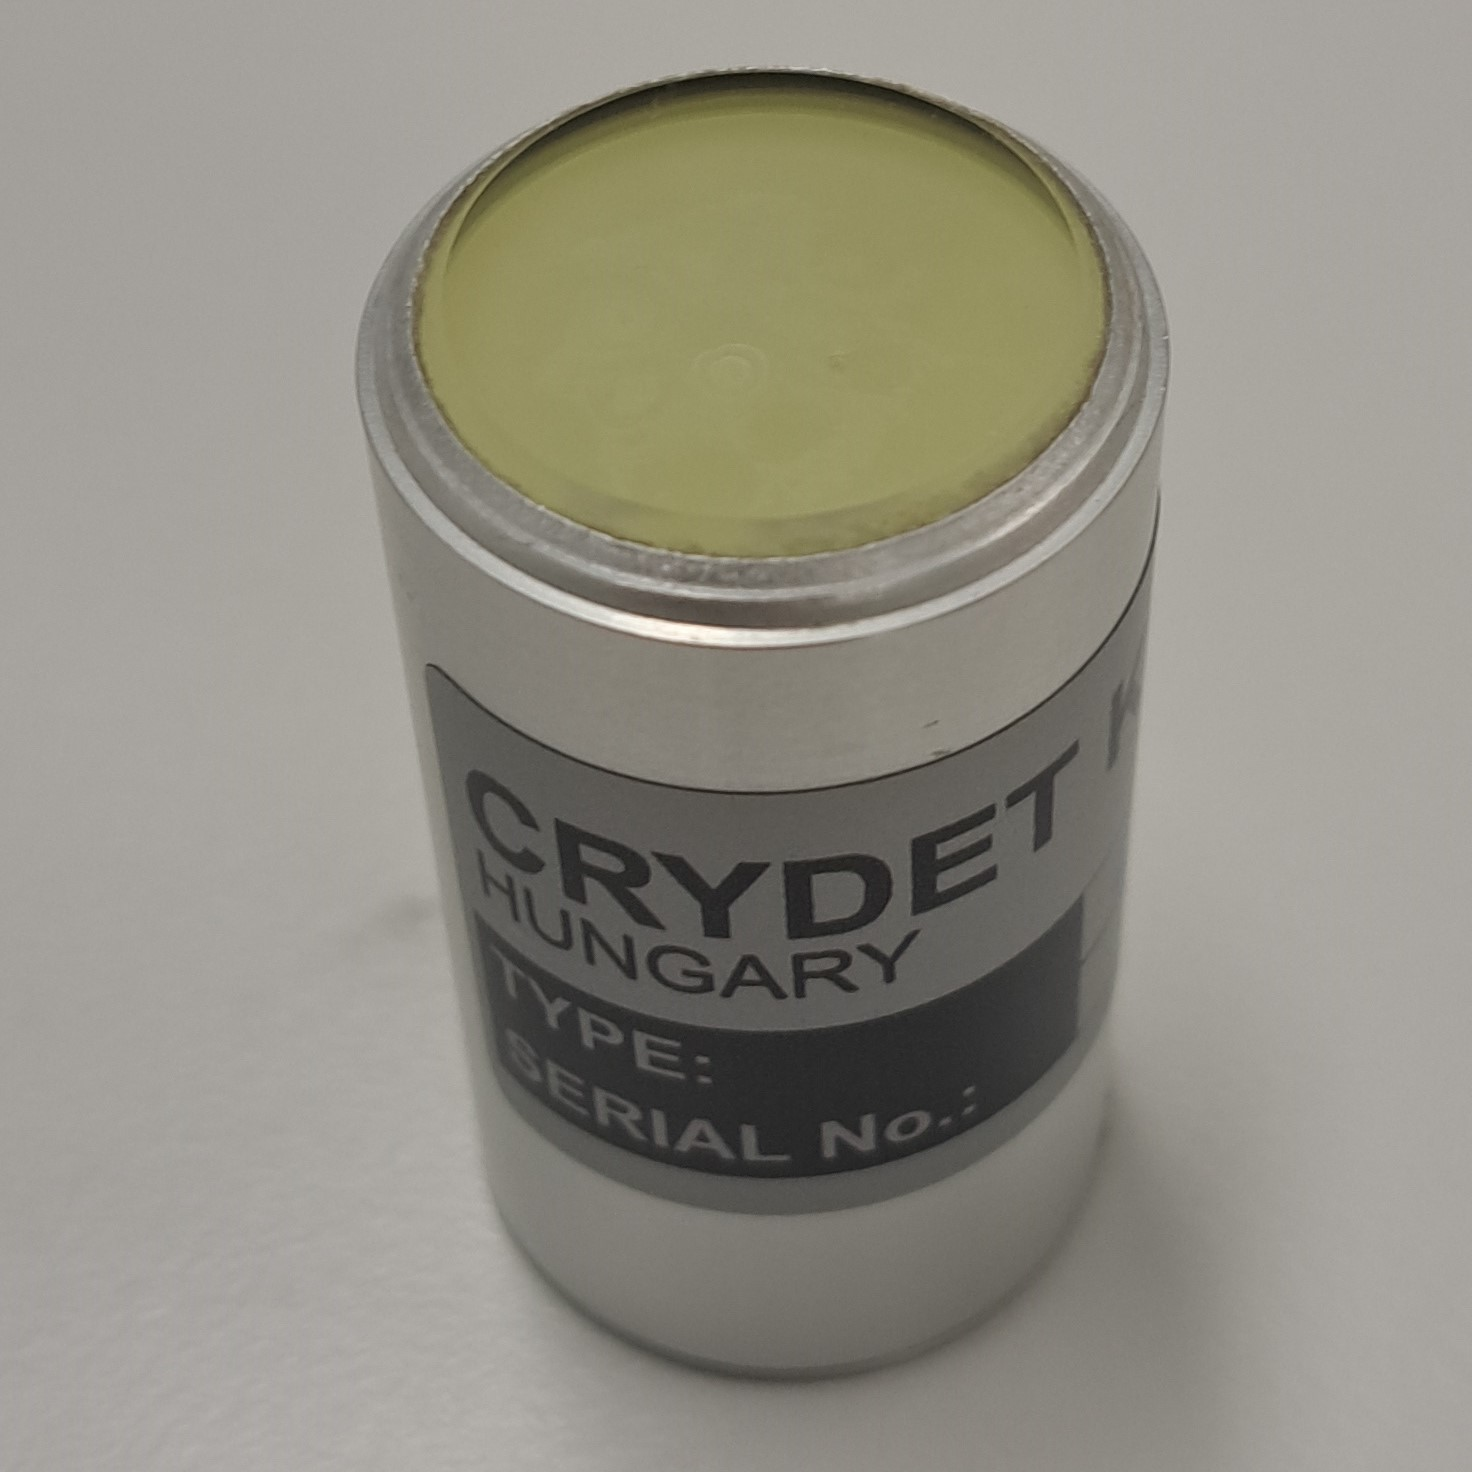
\includegraphics[trim=1cm 2cm 3cm 4cm, clip=true, totalheight=0.5\textheight, angle=90]{img/photo/Crystal.jpg}
        \caption[Photo d'un cristal NaI]{Photo d'un cristal NaI doper au thallium. Dimension~: diamètre 28*50~mm}
        \label{fig_Nai}
    \end{subfigure}
    \begin{subfigure}{0.45\textwidth}
        \centering
        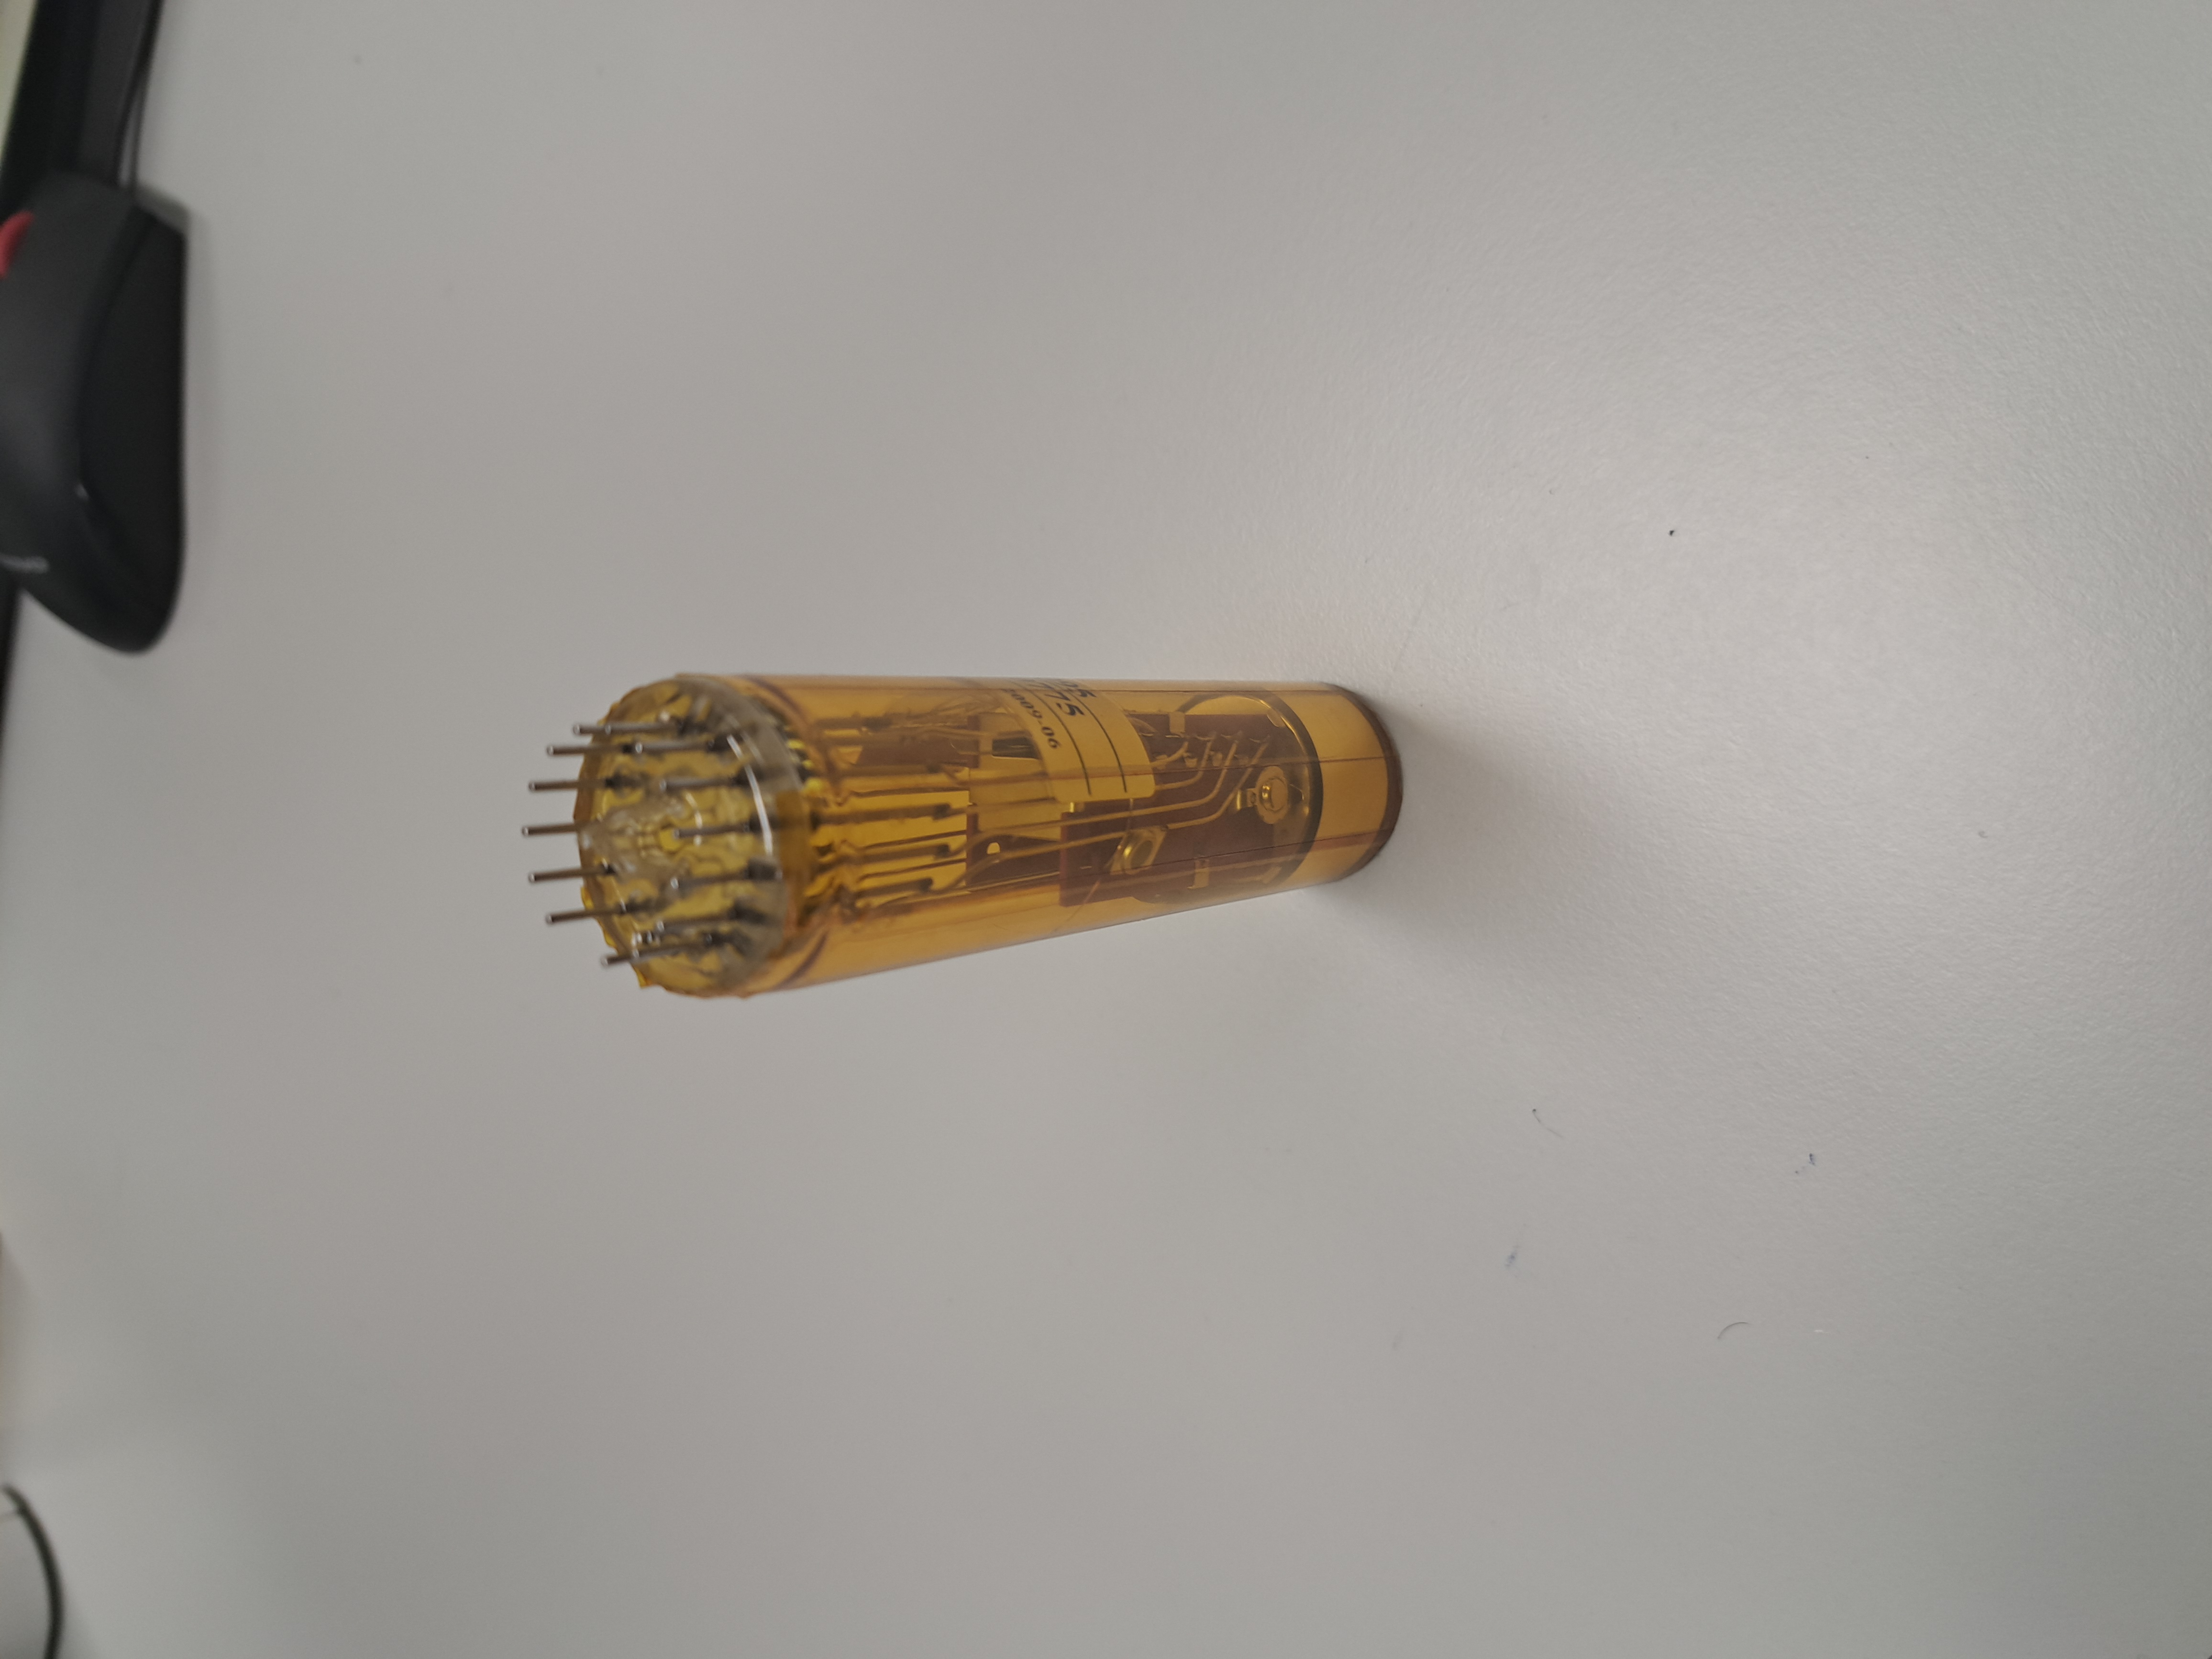
\includegraphics[width=0.7\textwidth]{img/photo/PMT.jpg}
        \caption[Photo d'un tube photomultiplicateur]{Photo d'un tube photomultiplicateur. Noter la fêlure à gauche de l'étiquette. Dimension~: diamètre 29*114~mm}
        \label{fig_PMT}
    \end{subfigure}
\end{figure}
\begin{description}
    \item[Un crystal NaI] Ce cristal a la propriété d'absorber les photons haut énergie des rayons gamma pour les réémettre comme des photons plus basse énergie (voir partie gauche de la \cref{fig_detecteur_gamma} et \cref{fig_Nai})~\cite{site:explication_NaI}
    \item[Un tube photomultiplicateur]ce tube permet de convertir un photon en un photoélectron qui est ensuite multiplié par le tube pour être converti en signaux électriques. (Voir partie droite de la \cref{fig_detecteur_gamma} et \cref{fig_PMT})~\cite{site:explication_NaI}
\end{description}
À la demande du client (Somaïr), une sonde basse a été incluse dans le projet pour permettre de faire des mesures aux niveaux du sol comme elle était faite avant (voir\ref{}). %photo et section
Les études internes montrent que les mesures les plus fiables sont faites à partir de la sonde haute donc la décision a été prise d'inclure les deux. À l'heure actuel, selon les données enregistrées par la sonde, 68,5~\% des mesures sont faits à partir de la sonde haute et 29~\% à partir de la sonde basse. Les autres mesures sont faites avec une combinaison des deux.

\subsection{Le GPS différentiel}
\label{ssec_Gps_differenciel}
Pour que la CanOp puisse fonctionner correctement, il faut qu'elle soit située très précisément ($\pm$ 10~cm sur les axes x et y et $\pm$ 1~cm sur les axes z), or un GPS classique n'arrive qu’a atteindre $\pm$~3~m horizontalement et $\pm$ 5~m verticalement dus notamment aux perturbations atmosphériques que subisse les signaux. 
\begin{figure}
    \centering
    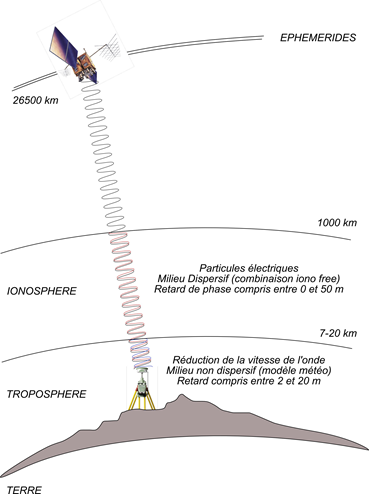
\includegraphics[height=0.5\textwidth]{img/she/GPS-mode-Naturel-5-10m.png}
    \caption[Source d'erreur des GPS]{Schéma présentant les sources d'erreur des GPS. Source~: Orphéon}
    \label{fig_GPS_error_source}
\end{figure}

Une des solutions possibles pour contourner ces problèmes est d'utiliser un GPS différentiel. Le principe de fonctionnement est simple, une station fixe à proximité de notre zone de mesure reçoit également les signaux GPS et en connaissant sa position précise peuvent calculer et transmettre les corrections nécessaires. \cite{site:GPS_diff}
\begin{figure}
    \centering
    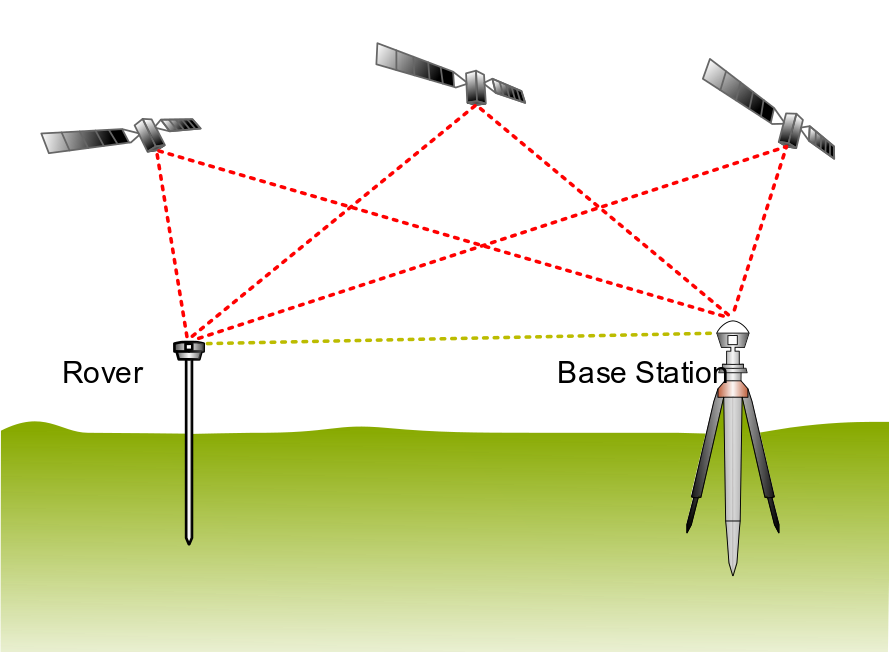
\includegraphics[width=0.5\textwidth]{img/she/Real_time_kinematic.png}
    \caption[Shema d'un systeme GPS differenciel]{Schéma d'un système GPS différentiel. Source~: \href{https://commons.wikimedia.org/wiki/File:Real_time_kinematic.svg}{TS Eriksson}, \href{https://creativecommons.org/licenses/by-sa/4.0}{CC BY-SA~4.0}, via Wikimedia Commons}
    \label{fig_RTK}
\end{figure}

\subsection{L'électronique}

    
\input{tex/Analyse_donnée}
\section{Amélioration de la CanOp}

Un des probleme majeur de la CanOp reste son poids relativement conséquent de 5,5~kg. Ce poids peut paraitre leger mais les operatuer doive porter les sonde a bout de bras pendant un shift de 8~hr sous le soleil avec une temperature qui monte regulierement au dessus de 40°C. Deja lors de sa conception on avez envisager de changer l'armature d'aluminum a de la fibre de carbon. 

Une grosse partie de mon travail a donc etait d'etudier et de proposer de solution a ce probleme. Assez rappidement trois avenue d'ameliration sont apparue.
\begin{enumerate}
    \item Alleger le gps 
    \item Alleger les sonde
    \item Repartir l'effort sur l'operateur
\end{enumerate}

\subsection{Allerger le Gps}
Actuellemnt le GPS est une piece monolitique fourit par Ophelia (voir \cref{ssec:Gps_differenciel}) qui calcule en interne la position corriger de la sonde. Une solution pourrait etre de fracturer le differnt partie du GPS et de delocaliser le calcule de la position et de sa correction a appliqué depuis la tablette de l'operateur en laissant l'antenne sur la sonde. D'autre solution a partir de puce integrer pourrait egalemetn mené a des econmie de poids.

\subsection{Alleger les sonde}
Les sonde sur les CanOp sont des sonde en deux piece composer d'un crystal scintilateur et d'un detectuer (ici un photomultiplier tube) (voir \cref{ssec:sonde}). C'est sonde sont relativement lourde et ne sont pas solidaire ce qui pose des problement de deconcetion accidentel et d'infiltration de poussiere/d'eau. 
J'ai donc chercher des sonde qui pourrait atre plus etanche et ou plus leger. En fesant c'est rechecher je suis tomber par accident sur des capteur solide state SiPM qui pourrait remplacer les tube photomultiplicateur. Ces composant sont devenue un remplacement viable de PMT que très recament et n'était donc pas diposible pour la V1 de la CanOp. C'est compossant present de nombreaux avantage:
\begin{itemize}
    \item plus leger
    \item peu cher a fabriquer en mass (capitalization sur les avancer faite en lithographie)
    \item moins cher
    \item Basse tenssion (5~V vs 1000-2000~V pour les PMT) $\rightarrow$ simplification des electronique
\end{itemize}

Ces avantage permet de produire des sonde gamma pesant 25~g\cite{} pour les plus petit comparer a environ 150~g\cite{} pour les sonde classic. Deplus ces sonde sont bien plus facile a rendre ettenche car il n'y a plus besoin de separer l'ecltronique du crystal.






\bibliographystyle{IEEEtran} % We choose the "plain" reference style
\bibliography{refs} % Entries are in the refs.bib file
\addcontentsline{toc}{section}{Biliography}
\clearpage


\appendix
\section{Bilan Personnel}

\end{document}


